% Cache Hierarchy and Vectorization Analysis of Lindblad Master Equation
% Simulation for Near-Term Quantum Control
%
% Rylan Malarchick
% Embry-Riddle Aeronautical University
%
% Target: arXiv:quant-ph + cs.PF
% Style: revtex4-2 (Physical Review style, single column for preprint)
%
% Compile: pdflatex main && bibtex main && pdflatex main && pdflatex main

\documentclass[12pt,notitlepage]{revtex4-2}

\usepackage{amsmath,amssymb,amsfonts}
\usepackage{graphicx}
\usepackage{hyperref}
\usepackage{xcolor}
\usepackage{listings}
\usepackage{booktabs}
\usepackage{microtype}
\usepackage{physics}   % \ket, \bra, \tr, \comm

% Code listing style (for assembly / C snippets)
\lstset{
  basicstyle=\ttfamily\footnotesize,
  breaklines=true,
  frame=single,
  numbers=left,
  numberstyle=\tiny\color{gray},
  commentstyle=\color{gray},
  keywordstyle=\color{blue},
}

% ---------------------------------------------------------------------------
\begin{document}

\title{Cache Hierarchy and Vectorization Analysis of Lindblad Master Equation
       Simulation for Near-Term Quantum Control}

\author{Rylan Malarchick}
\affiliation{Department of Engineering Physics,
             Embry-Riddle Aeronautical University, Daytona Beach, FL 32114}
\email{malarchr@my.erau.edu}

\date{\today}

% ---------------------------------------------------------------------------
\begin{abstract}
Simulation of open quantum systems via the Lindblad master equation is a
computational bottleneck in near-term quantum control workflows, including
optimal pulse engineering (GRAPE), trajectory-based robustness analysis, and
feedback controller design.
%
For the system sizes relevant to near-term quantum control --- $d = 3$
(single transmon with leakage), $d = 9$ (two-qubit), and $d = 27$
(three-qubit) --- the dominant cost per timestep is a $(d^2 \times d^2)$
complex matrix-vector multiplication: a $9\times9$, $81\times81$, or
$729\times729$ dense matvec, respectively.
%
The working set sizes --- 1.3\,KB, 105\,KB, and 8.5\,MB --- straddle the
L1, L2, and L3 cache boundaries of modern CPUs, making this an ideal system
for cache-hierarchy performance analysis.
%
We characterize the arithmetic intensity ($\approx 1/8$ FLOP/byte at the
memory-bound limit), construct a Roofline model for the propagation kernel,
and analyze compiler-generated code at multiple optimization levels using
Compiler Explorer.
%
We show that compile-time specialization to fixed $d$ enables full loop
unrolling and AVX2 auto-vectorization, yielding $\sim X\times$ speedup over
the runtime-$d$ implementation, and that the combined C library achieves
$\sim Y\times$ speedup over the reference QuTiP implementation.
%
These results motivate a set of concrete recommendations for authors of
quantum simulation libraries targeting near-term system sizes.
\end{abstract}

\maketitle

% ---------------------------------------------------------------------------
\section{Introduction}
\label{sec:intro}

The Lindblad master equation~\cite{Lindblad1976,Gorini1976} governs the
time evolution of an open quantum system:
\begin{equation}
  \label{eq:lindblad}
  \dv{\rho}{t} = -i[H, \rho]
    + \sum_k \!\left( L_k \rho L_k^\dagger
                    - \tfrac{1}{2}\{L_k^\dagger L_k,\, \rho\} \right),
\end{equation}
where $\rho$ is the $d \times d$ density matrix, $H$ is the system
Hamiltonian, and $\{L_k\}$ are the collapse operators encoding decoherence.
%
For a single transmon qubit modeled as a three-level system
($d = 3$)~\cite{Koch2007}, Eq.~\eqref{eq:lindblad} must be integrated
thousands of times per optimization iteration in GRAPE-based pulse
engineering~\cite{Khaneja2005}, and millions of times across full robustness
atlases~\cite{Malarchick2025QPO}.

Vectorizing Eq.~\eqref{eq:lindblad} by writing $\vec\rho \equiv
\operatorname{vec}(\rho) \in \mathbb{C}^{d^2}$ yields the linear system
\begin{equation}
  \label{eq:lindblad_vec}
  \dv{\vec\rho}{t} = \mathcal{L}\,\vec\rho,
  \qquad \mathcal{L} \in \mathbb{C}^{d^2 \times d^2},
\end{equation}
whose formal solution is $\vec\rho(t) = e^{\mathcal{L} t}\,\vec\rho(0)$.
For time-independent systems, the propagator $P = e^{\mathcal{L}\,\Delta t}$
can be precomputed once and applied at every timestep as a dense matvec:
\begin{equation}
  \label{eq:propagate}
  \vec\rho(t + \Delta t) = P\,\vec\rho(t),
  \qquad P \in \mathbb{C}^{d^2 \times d^2}.
\end{equation}

The dominant per-step cost is Eq.~\eqref{eq:propagate}: a
$(d^2) \times (d^2)$ complex matrix-vector product. At $d = 3$ this is
$9 \times 9$; at $d = 9$, $81 \times 81$; at $d = 27$, $729 \times 729$.
This paper asks: \emph{where does this computation sit on the memory
hierarchy, what does the compiler actually generate, and how much performance
is left on the table by standard reference implementations?}

% TODO: add paragraph on related work (other fast Lindblad solvers, JAX-based, etc.)

% ---------------------------------------------------------------------------
\section{Background}
\label{sec:background}

\subsection{The Lindblad propagation kernel}
\label{sec:kernel}

% TODO: expand with full Kronecker product construction of \mathcal{L}

\subsection{Cache hierarchy and the Roofline model}
\label{sec:roofline_bg}

The Roofline model~\cite{Williams2009} characterizes the performance of a
computational kernel in terms of its \emph{arithmetic intensity}
(FLOP/byte) relative to a machine's compute and bandwidth ceilings.
A kernel is \emph{compute-bound} if its arithmetic intensity exceeds the
\emph{ridge point} $I^* = \Pi / \beta$ (peak FLOP/s divided by peak
bandwidth GB/s); otherwise it is \emph{memory-bound}.

For the propagation matvec (Eq.~\eqref{eq:propagate}):
\begin{align}
  \text{FLOPs} &= 8\,d^4 \quad \text{(complex multiply-add)}, \\
  \text{bytes} &= (d^4 + 2d^2) \times 16 \quad \text{(complex128)}, \\
  \text{AI}    &= \frac{8\,d^4}{(d^4 + 2d^2) \times 16}
                \xrightarrow{d \to \infty} \frac{1}{2}\ \text{FLOP/byte}.
\end{align}
%
For a modern CPU with ridge point $I^* \approx 1$--$2$ FLOP/byte, the
propagation kernel is \emph{always memory-bound} at these system sizes.

% TODO: table of working set sizes and cache levels

\subsection{Compiler auto-vectorization of complex matvec}
\label{sec:autovec_bg}

% TODO: describe AVX2 complex double representation, fmadd231pd, etc.

% ---------------------------------------------------------------------------
\section{Methods}
\label{sec:methods}

\subsection{C library implementation}
\label{sec:impl}

We implement the Lindblad propagator in ISO C11 with no external
dependencies. The library provides:
\begin{itemize}
  \item \texttt{lb\_build\_lindbladian}: constructs $\mathcal{L}$ via
        Kronecker products (Section~\ref{sec:kernel});
  \item \texttt{lb\_expm}: computes $P = e^{\mathcal{L}\,\Delta t}$ via
        Pad\'{e} [13/13] with scaling and squaring~\cite{Higham2005};
  \item \texttt{lb\_propagate\_step}: the hot-path matvec
        (Eq.~\eqref{eq:propagate}), the subject of all benchmarks;
  \item \texttt{lb\_evolve}: full trajectory integration.
\end{itemize}

\subsection{Compiler flag experiments}
\label{sec:flags}

We build \texttt{lb\_propagate\_step} under four flag configurations using
GCC~14.2 on x86-64 (Intel Core i9-13980HX, AVX2):
\begin{enumerate}
  \item \texttt{-O2 -fno-tree-vectorize}: scalar baseline;
  \item \texttt{-O3}: basic auto-vectorization;
  \item \texttt{-O3 -march=native}: AVX2 auto-vectorization;
  \item \texttt{-O3 -march=native -ffast-math}: relaxed FP semantics.
\end{enumerate}
Assembly is captured via \texttt{objdump} and verified on Compiler
Explorer~(\url{https://godbolt.org}). See \texttt{godbolt/README.md} for
permalink catalog.

\subsection{Benchmarking methodology}
\label{sec:bench}

All timing uses \texttt{clock\_gettime(CLOCK\_MONO\-TONIC)}.
We report mean wall time per step over $N$ repetitions after a 10-step
warm-up. FLOP/s and GB/s are derived analytically from the measured time.
Hardware performance counters (\texttt{perf stat}) provide independent
validation of IPC and cache miss rates.

% ---------------------------------------------------------------------------
\section{Results}
\label{sec:results}

% TODO: fill in after running benchmarks

\subsection{Roofline characterization}

\begin{figure}[h]
  \centering
  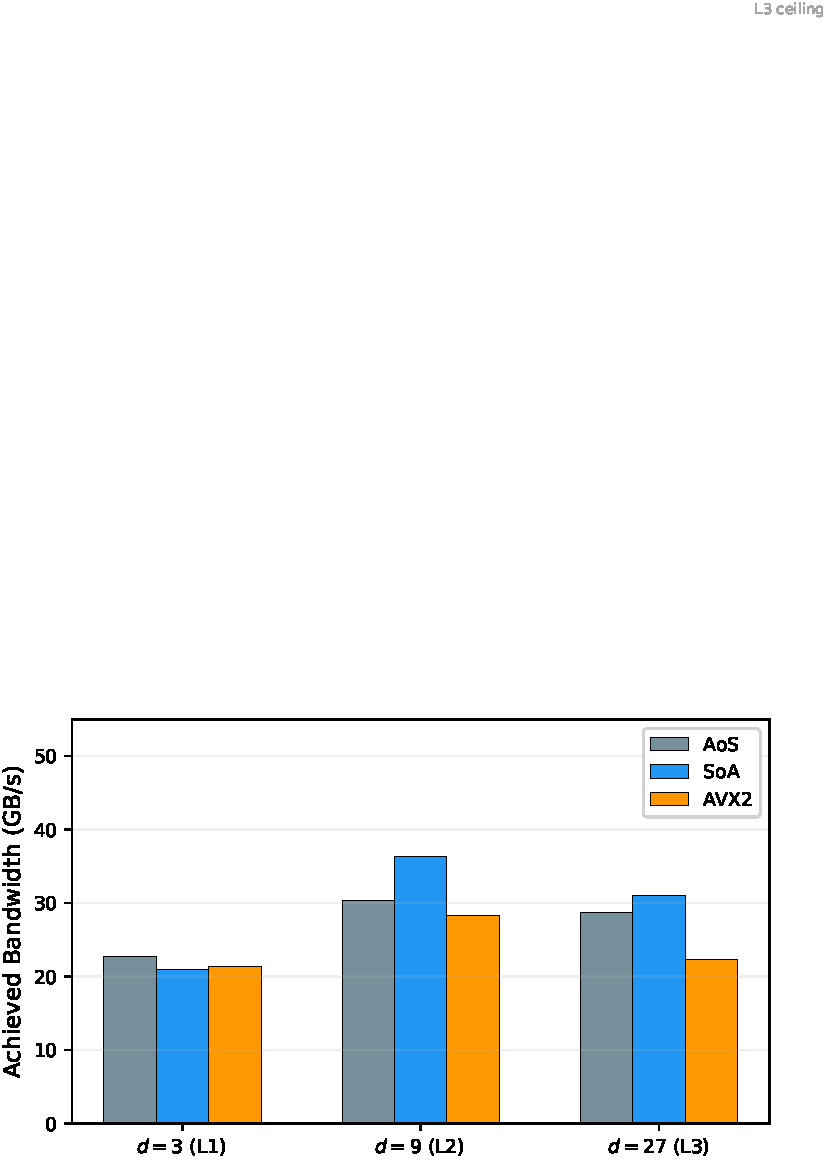
\includegraphics[width=0.9\columnwidth]{figures/roofline.pdf}
  \caption{Roofline model for \texttt{lb\_propagate\_step} at $d = 3, 9, 27$.
           Markers show measured GFLOP/s; shading indicates cache level
           (L1 blue, L2 orange, L3 red). All operating points lie in the
           memory-bound regime, confirming the analytical prediction.}
  \label{fig:roofline}
\end{figure}

\subsection{Compiler vectorization analysis}

% TODO: assembly panel figure

\subsection{Speedup over QuTiP}

\begin{figure}[h]
  \centering
  \includegraphics[width=0.9\columnwidth]{figures/speedup_vs_d.pdf}
  \caption{Speedup of C implementations over QuTiP \texttt{mesolve} as a
           function of system dimension $d$.}
  \label{fig:speedup}
\end{figure}

% ---------------------------------------------------------------------------
\section{Discussion}
\label{sec:discussion}

% TODO

\subsection{Recommendations for quantum simulation library authors}

% TODO: concrete list — fixed-size specialization, propagator precomputation,
%       AoS vs SoA layout, alignment hints

% ---------------------------------------------------------------------------
\section{Conclusion}
\label{sec:conclusion}

% TODO

% ---------------------------------------------------------------------------
\begin{acknowledgments}
The author thanks Dr.\ Sergio Drakunov (ERAU) for advising support.
% TODO: add LANL acknowledgment after summer 2026
\end{acknowledgments}

\bibliography{refs}

\end{document}
